\section{Results}

The expansion of researcher mobility concealed different forms of geographic inequality at the international and domestic scales. International flows became more evenly distributed across countries, but most increases in national shares were concentrated in a small subset of countries. Within countries, newly recorded cities contributed to rising concentration, while flows often became more even among cities recorded throughout the study. This cross-scale contrast occurred in all four disciplinary domains and was strongest in social sciences when the domestic comparison included the cities recorded each year.

\Needspace{4\baselineskip}
\subsection{Overall Equalization of International Mobility Masks Concentrated Growth in National Shares}

Although the overall distribution of international mobility became more even across countries, increases in national shares of global flows were highly concentrated among a small number of countries. A national share measures a country's combined international inflows and outflows as a proportion of the worldwide total. Between 1998 and 2025, the Herfindahl--Hirschman index (HHI), which gives greater weight to large shares, fell from 0.1016 to 0.0700, and the Gini coefficient, which summarizes disparities across national flow volumes, fell from 0.9022 to 0.8551. Of the 162 countries whose shares were higher in 2025 than in 1998, 44 accounted for 85.0\% of the sum of those increases in percentage points. These changes accompanied an increase in annual events from 154,323 to 938,401, with the latter 2.04 times the prediction obtained from the observed number of directed country pairs at the 1998 mean flow per pair (Fig.~\ref{fig:fig2}a,b). Thus, the diversification of scientific migration origins and destinations documented previously\cite{ref008} coexisted with a concentration of national share growth.

% The tall panel and its full caption can share a float page.
\begin{figure}[!tp]
\centering
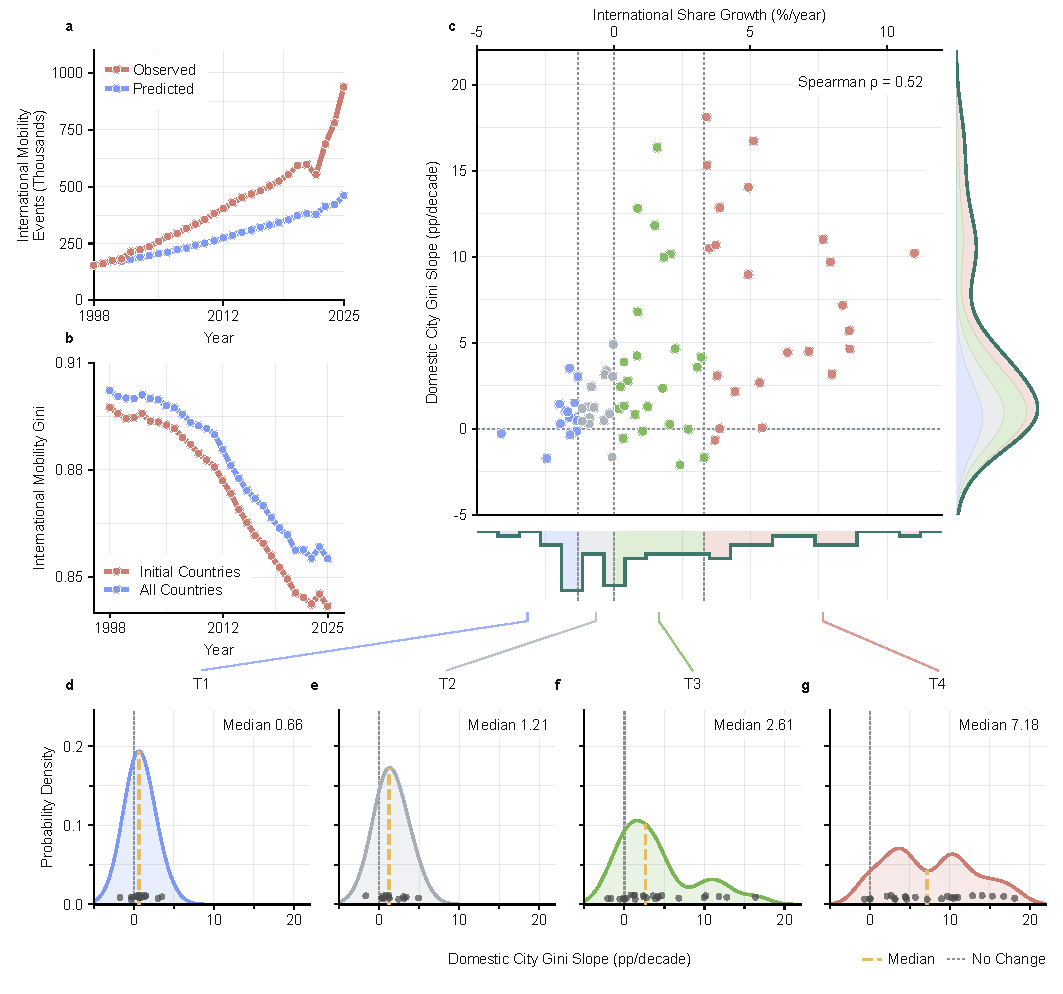
\includegraphics[width=\linewidth]{figures/Fig2.pdf}
\caption{\textbar\ \textbf{International Mobility Expansion And Cross-Scale Changes In Concentration.} \textbf{a,} Observed worldwide annual international mobility events (red) and the predicted total using each year's number of directed country pairs and the 1998 mean flow per pair (blue). \textbf{b,} Annual Gini of international mobility shares for the same 203 countries with recorded flows in every study year (Initial Countries, red) and for all countries with recorded flows in the plotted year (All Countries, blue). \textbf{c,} Fitted annual growth rates of countries' shares of worldwide international mobility (\%/year) and slopes of domestic city Gini (pp/decade) for the 76 countries assigned to T1--T4, with one point per country. Colours identify T1--T4: faster decline, slower decline, slower growth and faster growth, respectively (15, 14, 24 and 23 countries). Vertical dashed lines mark the group boundaries, the horizontal dashed line marks a zero Gini slope, and the annotation reports Spearman's $\rho$. The inverted histogram shows country counts by international-share growth. The right marginal curve shows the pooled density of domestic Gini slopes, with bands showing the contribution of each group weighted by its share of the 76 countries. Coloured guides link the groups to d--g. \textbf{d--g,} Kernel density estimates of Gini trends across annually recorded domestic cities in T1--T4, respectively. Dots represent countries, yellow dashed lines mark medians and grey vertical lines mark zero change. Inflows and outflows are combined. }
\label{fig:fig2}
\end{figure}

\begin{figure}[!htbp]
\centering
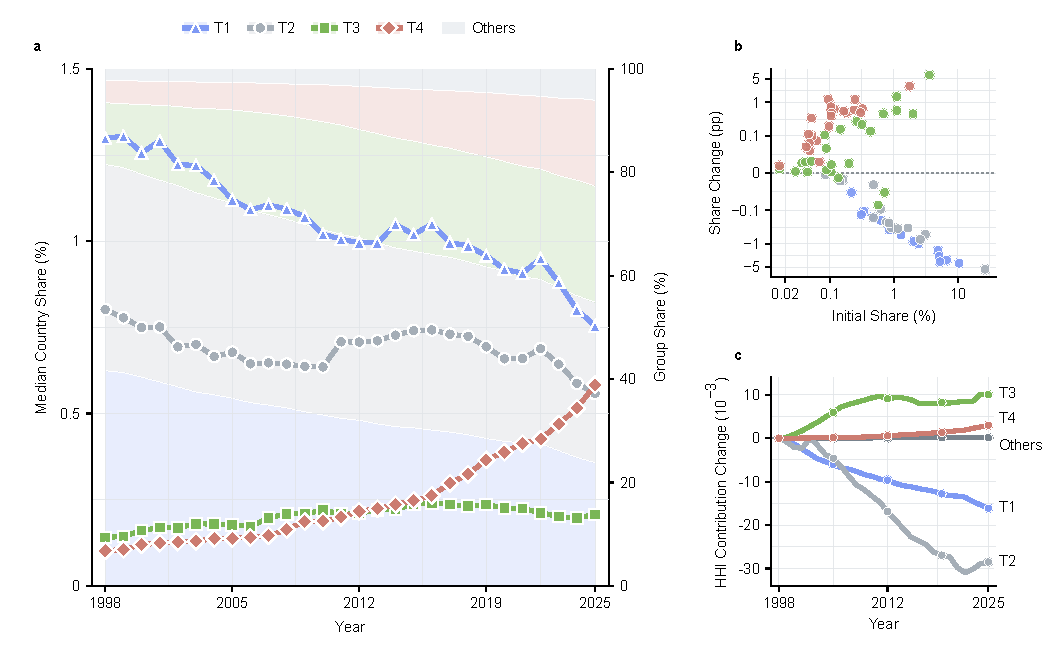
\includegraphics[width=\linewidth]{figures/Fig3.pdf}
\caption{\textbar\ \textbf{Redistribution Of International Mobility Across Countries.} \textbf{a,} Annual medians of individual countries' shares of worldwide international mobility within T1--T4 (lines and diamonds, left axis) and annual sums of country shares within each group, including Others (stacked bands, right axis). T1--T4 denote faster decline, slower decline, slower growth and faster growth in international shares, respectively, and contain 15, 14, 24 and 23 countries; Others includes countries outside this 76-country sample. \textbf{b,} Each point represents one of the 76 countries in T1--T4, using the same colours as in a. The horizontal axis shows the country's share of worldwide international mobility in 1998 on a logarithmic scale. The vertical axis shows its 1998--2025 change in percentage points (pp) on a symmetric logarithmic scale, linear between $-0.1$ and $+0.1$ pp. The dashed line marks zero change. \textbf{c,} Annual change from the 1998 baseline in each group's contribution to the Herfindahl--Hirschman index (HHI), calculated as the sum of squared worldwide shares of its countries. Axis values are expressed in units of $10^{-3}$. In each year, the five changes sum to the worldwide HHI change since 1998. }
\label{fig:fig3}
\end{figure}

The fastest-growing countries accounted for a large part of the increase in shares but remained the smallest group by combined share. For T1--T4, we estimated an annual percentage growth rate for each of the 76 countries with domestic data by fitting a straight line to the logarithm of each country's international share over all 28 years. Negative and positive growth rates were each split at their own unrounded median: T1 contains negative rates at or below the negative median, T2 the remaining negative rates, T3 positive rates at or below the positive median, and T4 the remaining positive rates. The groups represent faster decline, slower decline, slower growth and faster growth, respectively, and contain 15, 14, 24 and 23 countries (Fig.~\ref{fig:fig2}c). All 44 countries identified above belonged to T3 or T4. T4 alone accounted for 45.5\% of the summed share increases from 1998 to 2025. Its combined share rose from 4.39\% to 16.62\%, still the smallest of the four groups in 2025 (Fig.~\ref{fig:fig3}a,b).

Declining shares in T1 and T2 outweighed the concentrating contribution of growth in T3 and T4. The sum of squared national shares, which adds directly to worldwide HHI, fell by 0.0446 in T1 and T2 combined but rose by 0.0130 in T3 and T4 combined (Fig.~\ref{fig:fig3}c). Overall deconcentration thus reflected the redistribution of weight away from declining-share groups, alongside concentrated increases elsewhere. Both international HHI and Gini also fell when annual event counts were equalized by random subsampling and when membership was held to the same 203 countries, which carried more than 99.94\% of worldwide flows in every year (Fig.~\ref{fig:fig2}b). This distinguishes the source of the decline within the broader pattern of weakening dominance by the largest hubs and persistent network hierarchy reported previously\cite{yenilmez2026}.

Countries with faster international-share growth also tended to have steeper increases in inequality across their annually recorded domestic cities. Across the 76 countries, the association between fitted share growth and domestic Gini slopes was positive (Spearman $\rho=0.52$; Fig.~\ref{fig:fig2}c), and median Gini slopes rose from 0.66 percentage points per decade in T1 to 7.18 in T4 (Fig.~\ref{fig:fig2}d--g). This is an association between countries' long-term trajectories: in separate annual comparisons of inflows and outflows within countries, confidence intervals included zero after accounting for country and year effects. The T groups therefore connect international redistribution to a domestic distributional question: whether faster national share growth coincides with widening city disparities, extending earlier evidence of links between internal and international regional migration\cite{ref029}.

\FloatBarrier
\Needspace{4\baselineskip}
\subsection{The Addition of Newly Recorded Cities Drives Concentration in Domestic Mobility}

Domestic mobility reached more cities, but the distribution across those cities became more unequal relative to their expanding number. Across the 76 countries, the median number of cities with recorded domestic inflows or outflows rose from 16 to 46. The median equivalent city count---the number of equally weighted cities that would produce the observed HHI---also rose, from 4.90 to 7.20, and HHI fell in 74 countries. This effective expansion lagged behind the increase in recorded cities: the median ratio of equivalent to recorded city counts fell from 0.312 to 0.163, while median Gini rose from 0.633 to 0.749. In 63 countries, fitted trends combined a falling ratio with rising Gini, the joint pattern we classify as domestic concentration. These city-volume disparities differ from the declining inequality in population-weighted regional internal-migration rates reported in continental comparisons\cite{ref029}; expanding participation and concentration can occur together.

Newly recorded cities contributed most to the rise in Gini in the great majority of countries with increasing concentration. Initial cities had domestic flows recorded in both 1998 and the year being compared. They included continuously recorded cities, which had records in every study year, and intermittently recorded initial cities, which lacked records in some later years. Newly recorded cities first had domestic flows recorded after 1998 and entered a comparison in years when they had recorded flows. We separated the Gini trend among continuously recorded cities from the contributions of including intermittently recorded initial cities and newly recorded cities. Newly recorded cities made the largest positive contribution in 57 of the 63 countries. In 2025, these cities represented a median 50.0\% of recorded cities but only 8.7\% of combined domestic inflows and outflows. Across all 76 countries, their median contribution was +0.373 percentage points per year, compared with 0.000 for intermittently recorded initial cities and $-0.122$ for changes among continuously recorded cities. This composition-based explanation complements evidence of core--periphery structure in domestic researcher mobility\cite{ref032}: adding many low-flow cities can widen measured disparities without increasing inequality among persistent participants.

Including newly recorded cities raised domestic Gini trends across all four international-growth groups and strengthened the apparent cross-scale association. Among initial cities, median Gini changed little, from 0.633 to 0.632 (Fig.~\ref{fig:fig4}b). All-city slopes exceeded initial-city slopes in 69 of 76 countries, with a median paired difference of +0.197 percentage points per year; 38 countries switched from a negative initial-city slope to a positive all-city slope (Fig.~\ref{fig:fig5}a). The upward shift occurred in most countries within each T group (Fig.~\ref{fig:fig4}c), with the four cases showing different annual paths (Fig.~\ref{fig:fig5}b--e). The correlation between international-share growth and domestic Gini slopes weakened from $\rho=0.52$ for all cities to $\rho=0.13$ for initial cities. The long-term association was therefore much weaker when newly recorded cities were excluded, adding a qualification to comparisons of internal and international migration\cite{ref029}.

\begin{figure}[!htbp]
\centering
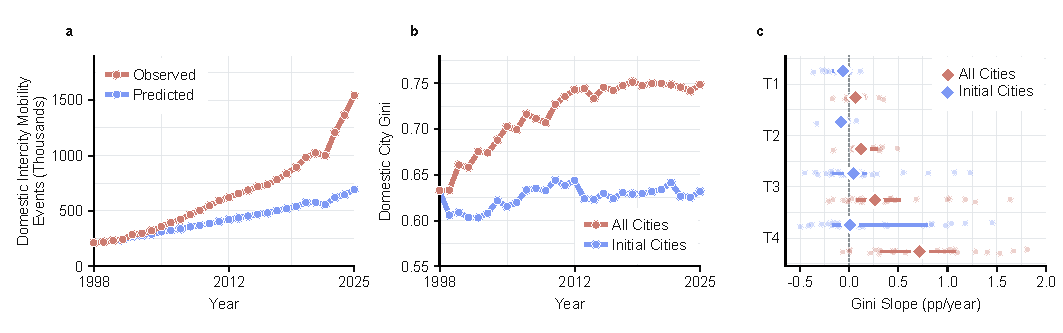
\includegraphics[width=\linewidth]{figures/Fig4.pdf}
\caption{\textbar\ \textbf{Expansion And Concentration Of Recorded Domestic Intercity Mobility.} \textbf{a,} Observed worldwide annual domestic intercity mobility events (red) and the predicted total using each year's number of directed within-country city pairs and the 1998 mean flow per pair (blue). \textbf{b,} Cross-country medians of annual domestic city Gini for the same 76 countries. All Cities (red) includes all cities with recorded flows that year. Initial Cities (blue) includes only cities recorded in 1998 that also had flows in the year being plotted. Both series use each included city's full domestic inflows and outflows. \textbf{c,} Country-level Gini slopes within T1--T4, with membership as in Fig.~\ref{fig:fig3} and city definitions as in b. Blue denotes initial cities and red denotes all recorded cities. Circles show all country values with small vertical offsets, large diamonds mark group medians, and horizontal coloured segments span the 25th to 75th percentiles. The vertical dashed line marks zero. Slopes use all 28 annual observations. Both b and c use the same 76 countries.}
\label{fig:fig4}
\end{figure}

\begin{figure}[!htbp]
\centering
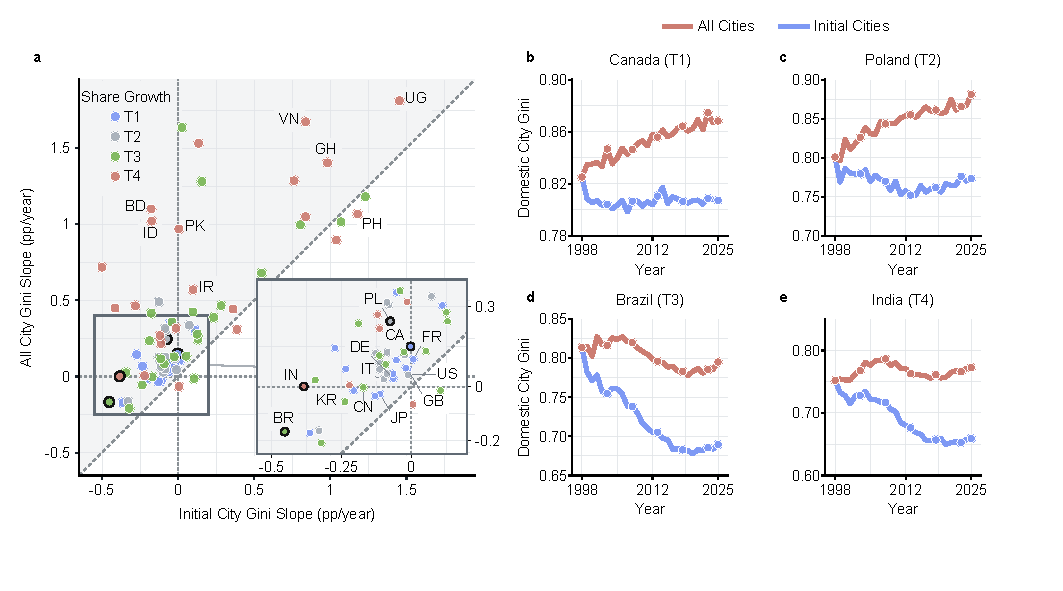
\includegraphics[width=\linewidth]{figures/Fig5.pdf}
\caption{\textbar\ \textbf{Changes In Domestic City Flow Distributions.} \textbf{a,} Fitted annual slopes of domestic city Gini for initial cities (horizontal axis) and all recorded cities (vertical axis), with one point per country ($n=76$). Colours identify T1--T4 as in Fig.~\ref{fig:fig3}. The diagonal dashed line marks equal slopes; the shaded region marks higher all-city slopes. Horizontal and vertical guides mark zero. The inset enlarges the boxed region. Black outlines identify the examples in b--e. Inset codes label the ten countries with the largest cumulative domestic event counts in the sample and the four examples. Additional codes identify selected peripheral points outside the inset region. \textbf{b--e,} Annual domestic city Gini for Canada (T1), Poland (T2), Brazil (T3) and India (T4), respectively. All Cities (red) includes all cities with recorded domestic flows that year. Initial Cities (blue) includes cities recorded in 1998 that also had flows in the year being plotted, using the same definition as Fig.~\ref{fig:fig4}b,c. Both series retain each included city's full domestic inflows and outflows and share one vertical axis within each country. Vertical scales vary by country. One country is selected within each of T1--T4 for the largest mean annual all-city minus initial-city Gini gap among group members with at least 100,000 domestic events overall, 1,000 in every year and 30 active cities in every year (Methods). Slopes are in percentage points (pp) per year.}
\label{fig:fig5}
\end{figure}

Cities recorded throughout the study often showed more even flow distributions even where the expanding city set became more concentrated. In 35 of the 63 countries with increasing all-city concentration, continuously recorded cities showed falling Gini and a rising equivalent count relative to their fixed number. These cities still carried a median 86.2\% of combined domestic flows in 2025 across the 76 countries. Each included city retained all its domestic inflows and outflows, including exchanges with cities outside the fixed list, so this comparison holds city membership constant while preserving its flow totals. This comparison extends earlier accounts of persistent urban mobility hierarchies\cite{ref031,ref032} by showing that disparities can narrow among the cities that carry most domestic flows.

The prevalence of rising domestic concentration depended strongly on the growth in recorded event volume. The 1.55 million domestic events observed in 2025 were 2.24 times the prediction based on the actual number of directed city pairs at the 1998 mean flow per pair (Fig.~\ref{fig:fig4}a), indicating that flows expanded beyond the increase in connections alone. When random subsampling held each country's annual event count constant, increasing concentration remained in 18 countries, compared with 63 in the full records, although city coverage still grew in 72 countries. Equal-event sampling\cite{gotelli2001} thus separates the persistent expansion of recorded participation from a more volume-sensitive increase in concentration.

\Needspace{4\baselineskip}
\subsection{Cross-Scale Contrasts in Flow Distributions Span All Four Disciplinary Domains and Are Strongest in Social Sciences}

International equalization and rising domestic city inequality coexisted in all four disciplinary domains when each year's recorded cities were included. International Gini declined in physical, life, health and social sciences, while domestic Gini rose in most countries in each domain within the same 45-country sample (Fig.~\ref{fig:fig6}a). This shared direction concerns the geographic distribution of flows across countries and within countries, extending disciplinary comparisons that have primarily distinguished researchers' mobility rates\cite{ref033}.

% Keep this figure on a page with the disciplinary results text.
\begin{figure}[!htb]
\centering
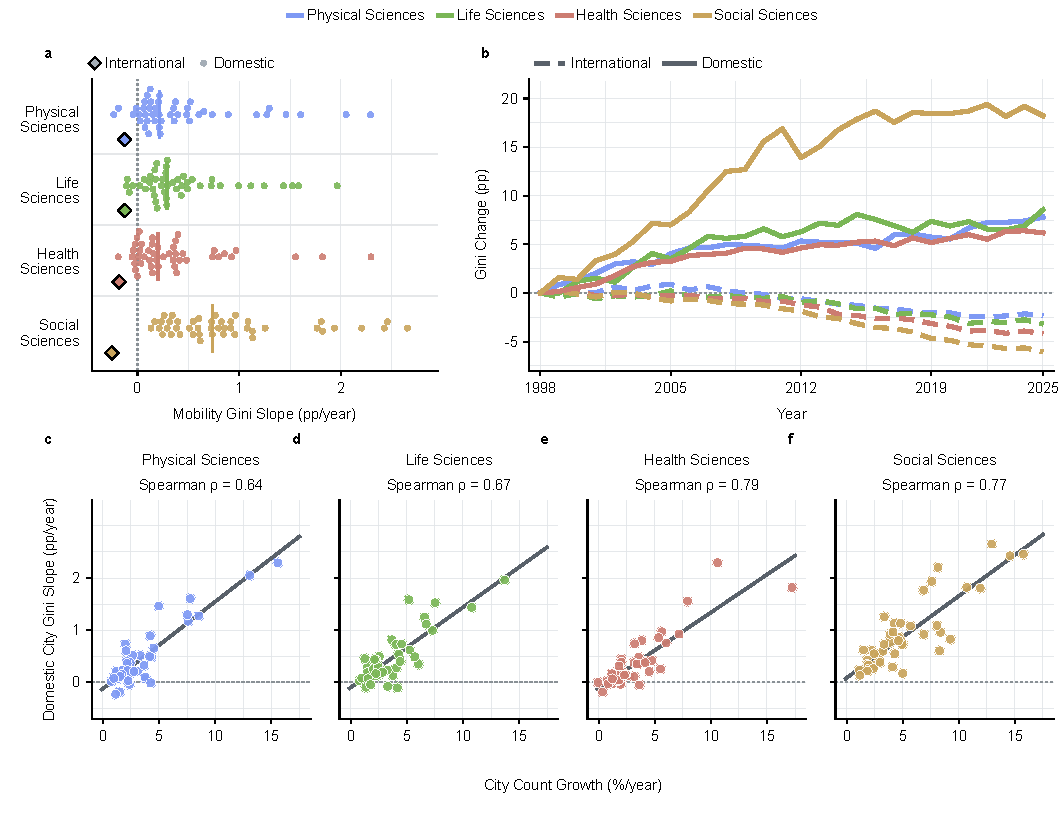
\includegraphics[width=\linewidth]{figures/Fig6.pdf}
\caption{\textbar\ \textbf{National Deconcentration And Domestic Urban Concentration Across Disciplines.} \textbf{a,} Fitted slopes of domestic city Gini (circles), their cross-country medians (vertical marks) and fitted slopes of international country Gini (diamonds). \textbf{b,} Dashed lines show annual changes in the Gini of international mobility across countries from the 1998 baseline. Solid lines show the cross-country medians of changes in domestic city Gini from each country's 1998 baseline. Colours identify the four disciplinary domains. \textbf{c--f,} Fitted annual growth in recorded city counts (horizontal) and domestic city Gini slopes (vertical) in physical, life, health and social sciences, respectively. Points represent countries. Grey lines show linear fits over a common horizontal range from \ensuremath{-}0.1\% to 17.5\% per year. Annotations report Spearman correlations. Domestic comparisons use the same 45 countries; international indices use all countries with flows in each domain and year. }
\label{fig:fig6}
\end{figure}

Social sciences showed the strongest cross-scale contrast, combining the steepest international Gini decline with the largest median domestic increase. Domestic Gini slopes were positive in all 45 countries, with a median of +0.74 percentage points per year, compared with +0.20--0.29 in the other domains; the international decline was 0.251 percentage points per year (Fig.~\ref{fig:fig6}a). By 2007, the median domestic increase from 1998 exceeded 10 percentage points in social sciences but remained below six in each other domain (Fig.~\ref{fig:fig6}b). The domain previously reported to have lower international mobility rates\cite{ref033} therefore showed the strongest redistribution of recorded flows in our comparisons, illustrating that mobility frequency and geographic redistribution describe different dimensions of change.

The exceptional domestic increase in social sciences reversed when the same cities were followed, as did the median trend in every other domain. Of the 45 countries in the disciplinary comparison, 34 each had at least two cities with domestic flows recorded in all four domains throughout all 28 years. In each of these 34 countries, we compared the trend based on each year's recorded cities with the trend based on a single city list shared across all four domains and years. Both calculations retained the full domestic inflows and outflows of each included city. With the fixed list, the median Gini slope changed from positive to negative in every domain. Social sciences showed the largest shift, from +0.600 to $-0.046$ percentage points per year. The +0.600 estimate uses each year's recorded cities in these 34 countries, while the +0.74 estimate above uses all 45 countries. The strongest observed domestic rise thus concerned an expanding city distribution, whereas continuously recorded cities showed a median shift towards more even flows in all four domains.

Growth in recorded city coverage was associated with rising domestic Gini in every domain, linking their common contrast to changes in participation. Across the same 45 countries, correlations between city-count growth and domestic Gini slopes ranged from Spearman $\rho=0.64$ to $0.79$ (Fig.~\ref{fig:fig6}c--f). Together with the fixed-city reversals, this indicates that the social-science extreme and the pattern shared across domains both depend on which cities enter the comparison. Differences in disciplinary mobility rates\cite{ref033} therefore coexist with a common distinction between widening participation and redistribution among persistent participants.

\FloatBarrier
